\documentclass{article}

\usepackage[english]{babel}
\usepackage[utf8]{inputenc}
\usepackage{amsmath,amssymb}
\usepackage{parskip}
\usepackage{graphicx}
\usepackage{tikz}
\usetikzlibrary{shapes,positioning}
\usepackage{multicol}
\usepackage{listings}

\lstdefinestyle{matlab}{
    language=Matlab,
    basicstyle=\ttfamily\small,
    numbers=left,
    numberstyle=\tiny,
    numbersep=5pt,
    frame=single,
    breaklines=true,
    breakatwhitespace=true,
    tabsize=4,
    captionpos=b,
    keywordstyle=\color{blue},
    commentstyle=\color{green},
    stringstyle=\color{red},
}




% Margins
\usepackage[top=2.5cm, left=3cm, right=3cm, bottom=4.0cm]{geometry}
% Colour table cells

% Get larger line spacing in table
\newcommand{\tablespace}{\\[1.25mm]}
\newcommand\Tstrut{\rule{0pt}{2.6ex}}         % = `top' strut
\newcommand\tstrut{\rule{0pt}{2.0ex}}         % = `top' strut
\newcommand\Bstrut{\rule[-0.9ex]{0pt}{0pt}}   % = `bottom' strut

%%%%%%%%%%%%%%%%%
%     Title     %
%%%%%%%%%%%%%%%%%
\title{Test Driven Development of a Feed Forward Neural Network}
\author{Fouad A.I. Azar}
\date{\today}

\begin{document}
\maketitle

\section{Propagation}

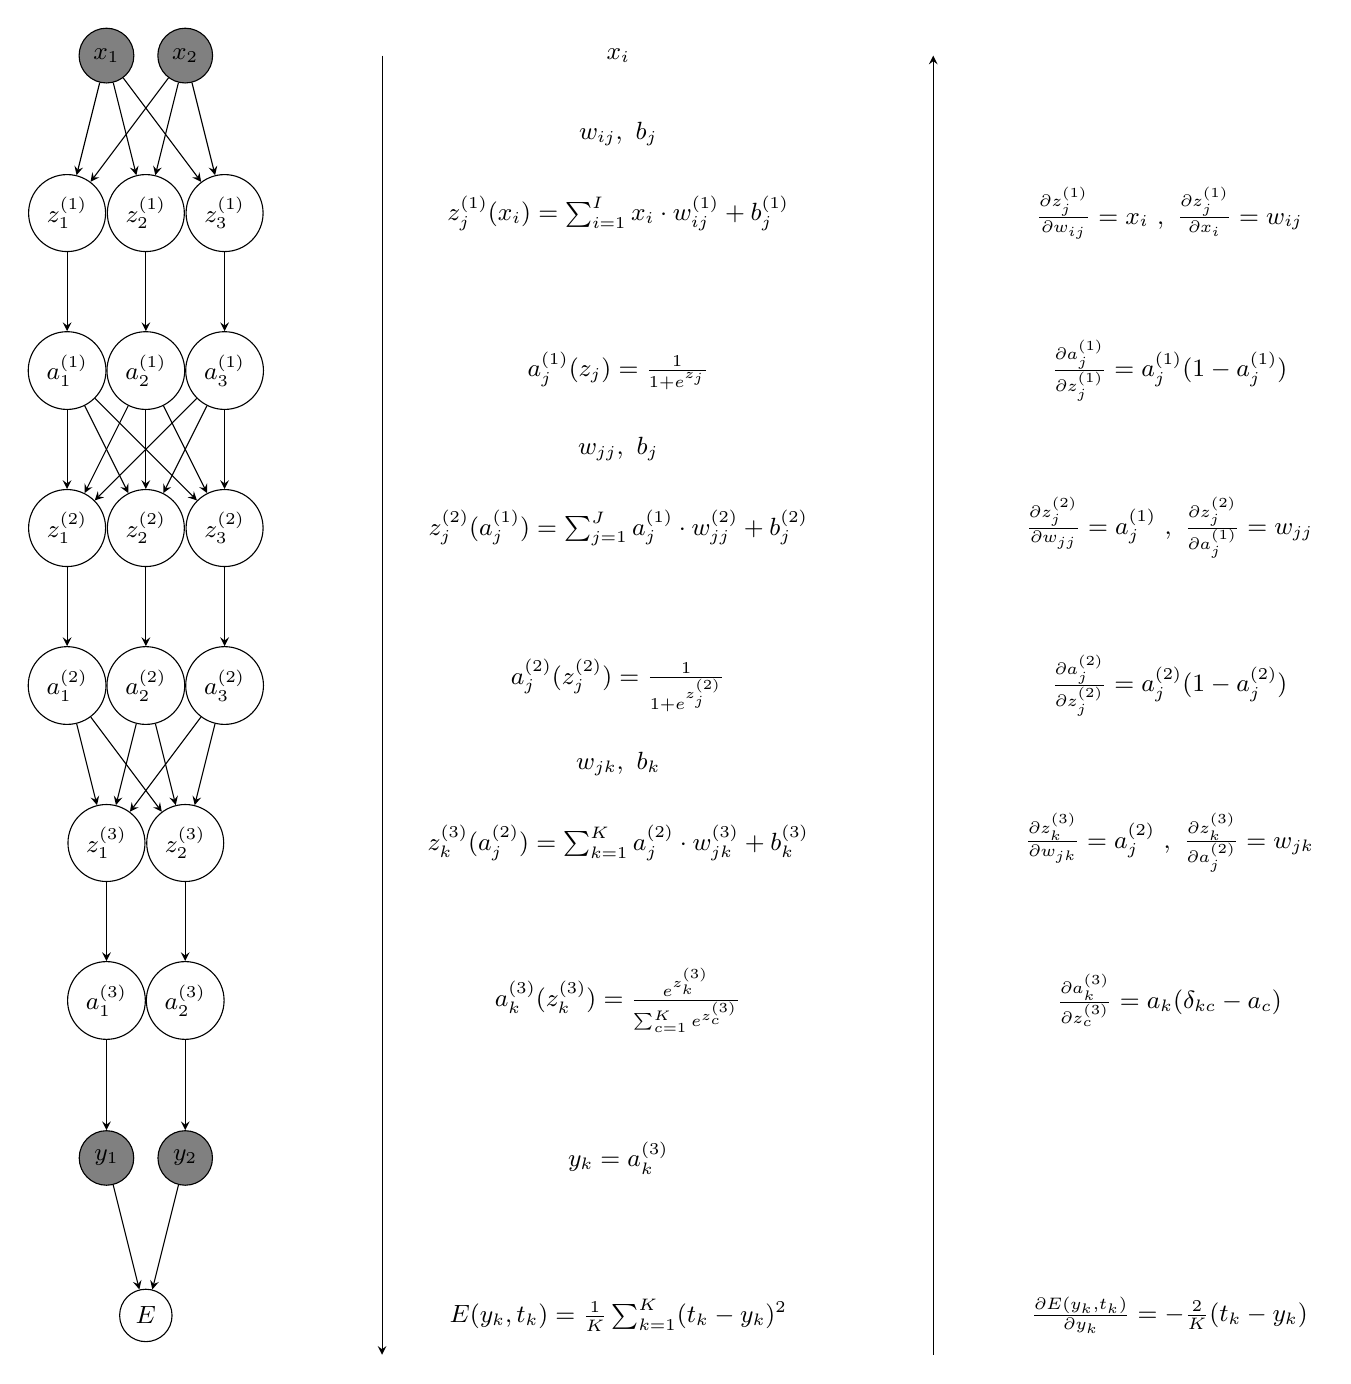
\begin{tikzpicture}[>=stealth]
\tikzstyle{every node}=[font=\small]

% Layer 1
\foreach \x in {1,2}
  \node[draw, circle, fill=gray] (x\x) at (\x+0.5, 10) {$x_{\x}$};
  \node at (8,10) {$x_i$};
  \node at (8,9) {$w_{ij}, \ b_j$};
% Layer 2
\foreach \y in {1,2,3}
  \node[draw, circle, minimum size=0.01cm] (z1\y) at (\y, 8) {$z^{(1)}_{\y}$};
\foreach \x in {1,2}
  \foreach \y in {1,2,3}
    \draw[->] (x\x) -- (z1\y);
  \node at (8,8) {$z^{(1)}_j(x_i) = \sum^I_{i=1} x_i\cdot w^{(1)}_{ij} + b^{(1)}_j$};
  \node at (15,8) {$\frac{\partial z^{(1)}_j}{\partial w_{ij}} = x_i \ , \ \frac{\partial z^{(1)}_j}{\partial x_i} = w_{ij}$};
% Layer 3
\foreach \y in {1,2,3}
  \node[draw, circle] (a1\y) at (\y, 6) {$a^{(1)}_{\y}$};
\foreach \y in {1,2,3}
  \draw[->] (z1\y) -- (a1\y);
  \node at (8,6) {$a^{(1)}_j(z_j) = \frac{1}{1+e^{z_j}}$};
  \node at (8,5) {$w_{jj}, \ b_j$};
  \node at (15,6) {$\frac{\partial a^{(1)}_j}{\partial z^{(1)}_j} = a^{(1)}_j(1-a^{(1)}_j)$}; 
% Layer 4
\foreach \y in {1,2,3}
  \node[draw, circle] (z2\y) at (\y, 4) {$z^{(2)}_{\y}$};
\foreach \y in {1,2,3}
  \foreach \z in {1,2,3}
    \draw[->] (a1\y) -- (z2\z);
  \node at (8,4) {$z^{(2)}_j(a^{(1)}_j) = \sum^J_{j=1} a^{(1)}_j\cdot w^{(2)}_{jj} + b^{(2)}_j$};
  \node at (15,4) {$\frac{\partial z^{(2)}_j}{\partial w_{jj}} = a_j^{(1)} \ , \ \frac{\partial z^{(2)}_j}{\partial a^{(1)}_j} = w_{jj}$};
% Layer 5
\foreach \y in {1,2,3}
  \node[draw, circle] (a2\y) at (\y, 2) {$a^{(2)}_{\y}$};
\foreach \y in {1,2,3}
  \draw[->] (z2\y) -- (a2\y);
  \node at (8,2) {$a^{(2)}_j(z^{(2)}_j) = \frac{1}{1+e^{z^{(2)}_j}}$};
  \node at (8,1) {$w_{jk}, \ b_k$};
  \node at (15,2) {$\frac{\partial a^{(2)}_j}{\partial z^{(2)}_j} = a^{(2)}_j(1-a^{(2)}_j)$};  
% Layer 6
\foreach \y in {1,2}
  \node[draw, circle] (z3\y) at (\y+0.5, 0) {$z^{(3)}_{\y}$};
\foreach \y in {1,2,3}
  \foreach \z in {1,2}
    \draw[->] (a2\y) -- (z3\z);
  \node at (8,0) {$z^{(3)}_k(a^{(2)}_j) = \sum^K_{k=1} a^{(2)}_j\cdot w^{(3)}_{jk} + b^{(3)}_k$};
  \node at (15,0) {$\frac{\partial z^{(3)}_k}{\partial w_{jk}} = a_j^{(2)} \ , \ \frac{\partial z^{(3)}_k}{\partial a^{(2)}_j} = w_{jk}$};

% Layer 7
\foreach \y in {1,2}
  \node[draw, circle] (a3\y) at (\y+0.5, -2) {$a^{(3)}_{\y}$};
\foreach \y in {1,2}
  \draw[->] (z3\y) -- (a3\y);
  \node at (8,-2) {$a^{(3)}_k(z^{(3)}_k) = \frac{e^{z^{(3)}_k}}{\sum^K_{c=1}e^{z^{(3)}_c}}$};
  \node at (15,-2) {$\frac{\partial a^{(3)}_k}{\partial z^{(3)}_c} = a_k(\delta_{kc} - a_c)$};
% Layer 8
\foreach \x in {1,2}
  \node[draw, circle, fill=gray] (y\x) at (\x+0.5, -4) {$y_{\x}$};
\foreach \x in {1,2}
    \draw[->] (a3\x) -- (y\x);
    \node at (8,-4) {$y_k = a^{(3)}_k$};

% Layer 9
\node[draw, circle, fill=white] (E) at (2, -6) {$E$};
\node at (8,-6) {$E(y_k,t_k) = \frac{1}{K}\sum_{k=1}^K (t_k - y_k)^2$};
\node at (15,-6) {$\frac{\partial E(y_k,t_k)}{\partial y_k} = -\frac{2}{K} (t_k - y_k)$};

% Connect the last layer to E
\foreach \x in {1,2}
  \draw[->] (y\x) -- (E);

  \draw[->] (5,10) -- (5,-6.5);
  \draw[->](12,-6.5) -- (12,10);
\end{tikzpicture}



\newpage
\section{Forward Propagation}
\subsection{Input Layer}
Let's start with an input column\footnote{indicated with ()} vector $x_i \in \mathbb{R}^I$ :
\begin{equation*}
    x_i = (1, 1)
\end{equation*}

and let's initialize a weight matrix of a non-random pattern such as $\{\forall i,j : w_{ij} =  0.5 \}$. Keep in mind the dimensions of the weight matrix is the cardinality\footnote{aka the number of nodes} of the input layer and the adjacent hidden layer ($J=3$):
\begin{equation*}
    w_{ij} =
            \begin{bmatrix}
            0.5 & 0.5 & 0.5 \\
            0.5 & 0.5 & 0.5 \\
            \end{bmatrix}
\end{equation*}

along with a bias column vector with cardinality $J$:
\begin{equation*}
    b_j = (1,1,1)
\end{equation*}
\subsection{Hidden Layer 1}
With these values defined, we can compute the values of the column vector $z^{(1)}$:
\begin{align*}
    z^{(1)}_j(x_i) &= \sum^I_{i=1} x_i\cdot w^{(1)}_{ij} + b^{(1)}_j\\ \\
    z_1 &= (x_1\cdot w_{11}) + (x_2\cdot w_{21}) + b_1 \\
    z_2 &= (x_1\cdot w_{12}) + (x_2\cdot w_{22}) + b_2\\
    z_3 &= (x_1\cdot w_{13}) + (x_2\cdot w_{23}) + b_3\\ \\
    z_1 &= (0.5) + (0.5) + 1 = 2\\ 
    z_2 &= (0.5) + (0.5) + 1 = 2\\ 
    z_3 &= (0.5) + (0.5) + 1 = 2\\  \\
    z^{(1)}_j &= (2, 2, 2)  
\end{align*}

Although this calculation is correction, it is extremely tedious. Let's use matrix multiplication instead:
\begin{align*}
    z^{(1)} &= 
    \underbrace{
    \begin{bmatrix}
        w_{11} & w_{12} & w_{13} \\
        w_{21} & w_{22} & w_{23} \\
    \end{bmatrix}^T
    }_{2\times 3}
    \cdot
    \underbrace{
    \begin{pmatrix}
        x_1 \\
        x_2 \\
    \end{pmatrix}
    }_{2\times 1}
    +
    \underbrace{
    \begin{pmatrix}
        b_1 \\
        b_2 \\
        b_3 \\
    \end{pmatrix}
    }_{3\times 1}\\
    &=
    \underbrace{
    \begin{bmatrix}
    w_{11} & w_{21} \\
    w_{12} & w_{22} \\
    w_{13} & w_{23} \\
    \end{bmatrix}
    \cdot
    \begin{pmatrix}
        x_1 \\
        x_2 \\
    \end{pmatrix}
    }_{3\times 1}
    +
    \underbrace{
    \begin{pmatrix}
        b_1 \\
        b_2 \\
        b_3 \\
    \end{pmatrix}
    }_{3\times 1}\\
    &=
    \begin{pmatrix}
        w_{11}x_1 + w_{21}x_2\\
        w_{12}x_1 + w_{22}x_2\\
        w_{13}x_1 + w_{23}x_2\\
    \end{pmatrix}
    +
    \begin{pmatrix}
        b_1\\
        b_2\\
        b_3\\
    \end{pmatrix}\\ \\
    &=
    \begin{pmatrix}
        w_{11}x_1 + w_{21}x_2+b_1\\
        w_{12}x_1 + w_{22}x_2+b_2\\
        w_{13}x_1 + w_{23}x_2+b_3\\
    \end{pmatrix}\\ \\
    &=(2,2,2)
\end{align*}

Let's write out this code in MATLAB and display the results here:

\begin{lstlisting}[style=matlab, label=your-label]
x = [1;1];
w = [...
    0.5,0.5,0.5;...
    0.5,0.5,0.5...
    ];
b = [1;1;1];

z_1 = w'*x +b %results show (2;2;2)
\end{lstlisting}

We'll now directly transfer $z_j^{(1)}$ to $a_j^{(1)}$ over a weightless connection. $a_j^{(1)}$ is a sigmoid function that will compute the $sig(z_j^{(1)})$ for each element. Therefore the resulting matrix should possess the same dimensionality as $z^{(1)}_j$.

\begin{align*}
    a_1^{(1)} &= \frac{1}{1+e^{-z_1}} = 0.8808\\
    a_2^{(1)} &= \frac{1}{1+e^{-z_2}} = 0.8808\\
    a_3^{(1)} &= \frac{1}{1+e^{-z_3}} = 0.8808\\
    a_j^{(1)} &= (0.8808,0.8808,0.8808)
\end{align*}

\begin{lstlisting}[style=matlab, label=your-label]
a_1 = 1./(1+exp(-z_1)) % results show(0.8808;0.8808;0.8808)
\end{lstlisting}

Before moving onto the next layer,
let's initialize a weight matrix of a non-random pattern such as $\{\forall j,j : w_{jj} =  0.5 \}$:
\begin{equation*}
    w_{jj} =
            \begin{bmatrix}
            0.5 & 0.5 & 0.5 \\
            0.5 & 0.5 & 0.5 \\
            0.5 & 0.5 & 0.5 \\
            \end{bmatrix}
\end{equation*}

along with a bias column vector with cardinality $J$:
\begin{equation*}
    b_j = (1,1,1)
\end{equation*}

\subsection{Hidden Layer 2}
We're now going to calculate the sum as we did previously, but this time, we'll get straight to the point:
\begin{align*}
    z^{(2)}_j(a^{(1)}_j) &= \sum^J_{j=1} a^{(1)}_j\cdot w^{(2)}_{jj} + b^{(2)}_j\\ \\
    z_1 &= (a_1 \cdot w_{11}) + (a_2 \cdot w_{21}) + (a_3 \cdot w_{31}) + b_1 \\
    z_2 &= (a_1 \cdot w_{12}) + (a_2 \cdot w_{22}) + (a_3 \cdot w_{32}) + b_2 \\
    z_3 &= (a_1 \cdot w_{13}) + (a_2 \cdot w_{23}) + (a_3 \cdot w_{33}) + b_3 \\ \\    
    z_1 &= (0.4404) + (0.4404) + (0.4404) + 1 = 2.3212\\ 
    z_2 &= (0.4404) + (0.4404) + (0.4404) + 1 = 2.3212\\
    z_3 &= (0.4404) + (0.4404) + (0.4404) + 1 = 2.3212\\
    z^{(2)}_j &= (1.8808, 1.8808, 1.8808)\\
    z^{(2)} &= 
    \underbrace{
    \begin{bmatrix}
        w_{11} & w_{12} & w_{13} \\
        w_{21} & w_{22} & w_{23} \\
        w_{31} & w_{32} & w_{33} \\
    \end{bmatrix}^T
    }_{3\times 3}
    \cdot
    \underbrace{
    \begin{pmatrix}
        a^{(1)}_1 \\
        a^{(1)}_2 \\
        a^{(1)}_3 \\
    \end{pmatrix}
    }_{3\times 1}
    +
    \underbrace{
    \begin{pmatrix}
        b_1 \\
        b_2 \\
        b_3 \\
    \end{pmatrix}
    }_{3\times 1}\\
    &=
    \underbrace{
    \begin{bmatrix}
        w_{11} & w_{21} & w_{31} \\
        w_{12} & w_{22} & w_{32} \\
        w_{13} & w_{23} & w_{33} \\
    \end{bmatrix}
    \cdot
    \begin{pmatrix}
        a^{(1)}_1 \\
        a^{(1)}_2 \\
        a^{(1)}_3 \\
    \end{pmatrix}
    }_{3\times 1}
    +
    \underbrace{
    \begin{pmatrix}
        b_1 \\
        b_2 \\
        b_3 \\
    \end{pmatrix}
    }_{3\times 1}\\ \\
    &=
    \begin{pmatrix}
        w_{11}a_1 + w_{21}a_2 + w_{31}a_3 \\
        w_{12}a_1 + w_{22}a_2 + w_{32}a_3 \\
        w_{13}a_1 + w_{23}a_2 + w_{33}a_3 \\
    \end{pmatrix}
    +
    \begin{pmatrix}
        b_1\\
        b_2\\
        b_3
    \end{pmatrix}\\ \\
    &=
    \begin{pmatrix}
        w_{11}a_1 + w_{21}a_2 + w_{31}a_3 + b_1\\
        w_{12}a_1 + w_{22}a_2 + w_{32}a_3 + b_2\\
        w_{13}a_1 + w_{23}a_2 + w_{33}a_3 + b_3\\
    \end{pmatrix}
     = (2.3212,2.3212,2.3212)
\end{align*}

and the snippet of code to validate
\begin{lstlisting}[style=matlab, label=your-label]
w_jj = [...
    0.5,0.5,0.5;...
    0.5,0.5,0.5;...
    0.5,0.5,0.5
    ];
b_2 = [1;1;1];

z_2 = w_jj'*a_1 + b_2 
\end{lstlisting}

We'll now directly transfer $z_j^{(2)}$ to $a_j^{(2)}$ over a weightless connection. $a_j^{(2)}$ is a sigmoid function that will compute the $sig(z_j^{(2)})$ for each element. Therefore the resulting matrix should possess the same dimensionality as $z^{(2)}_j$.

\begin{align*}
    a_1^{(2)} &= \frac{1}{1+e^{-z_1}} = 0.9106\\
    a_2^{(2)} &= \frac{1}{1+e^{-z_2}} = 0.9106\\
    a_3^{(2)} &= \frac{1}{1+e^{-z_3}} = 0.9106\\
    a_j^{(2)} &= (0.8808,0.8808,0.8808)
\end{align*}

\begin{lstlisting}[style=matlab, label=your-label]
a_2 = 1./(1+exp(-z_2)) % results show(0.9106;0.9106;0.9106)
\end{lstlisting}

Before moving onto the next layer, let's initialize a weight matrix of a non-random pattern such as $\{\forall j,k : w_{jk} =  0.5 \}$:
\begin{equation*}
    w_{jk} =
            \begin{bmatrix}
            0.5 & 0.5 \\
            0.5 & 0.5 \\
            0.5 & 0.5 
            \end{bmatrix}
\end{equation*}

along with a bias column vector with cardinality $K$:
\begin{equation*}
    b_k = (1,1)
\end{equation*}

\subsection{Output Layer}
We're now going to calculate the sum as we did previously, but this time, we'll get straight to the point:
\begin{align*}
    z^{(3)}_k(a^{(2)}_j) &= \sum^J_{j=1} a^{(2)}_j\cdot w^{(3)}_{jk} + b^{(2)}_k\\ \\
    z_1 &= (a_1 \cdot w_{11}) + (a_2 \cdot w_{21}) + (a_3 \cdot w_{31})+ b_1 \\     
    z_2 &= (a_1 \cdot w_{12}) + (a_2 \cdot w_{22}) + (a_3 \cdot w_{32})+ b_2 \\ \\   
    z_1 &= (0.4553) + (0.4553) + (0.4553)  + 1 = 2.3659\\ 
    z_2 &= (0.4553) + (0.4553) + (0.4553)  + 1 = 2.3659\\ 
    z^{(3)}_k &= (2.3659, 2.3659)\\ \\
    z^{(3)} &= 
    \underbrace{
    \begin{bmatrix}
        w_{11} & w_{12} \\
        w_{21} & w_{22} \\
        w_{31} & w_{32} \\
    \end{bmatrix}^T
    }_{3\times 2}
    \cdot
    \underbrace{
    \begin{pmatrix}
        a^{(1)}_1 \\
        a^{(1)}_2 \\
        a^{(1)}_3 \\
    \end{pmatrix}
    }_{3\times 1}
    +
    \underbrace{
    \begin{pmatrix}
        b_1 \\
        b_2 \\
    \end{pmatrix}
    }_{2\times 1}\\
    &=
    \underbrace{
    \begin{bmatrix}
        w_{11} & w_{21} & w_{31} \\
        w_{12} & w_{22} & w_{32} \\
    \end{bmatrix}
    \cdot
    \begin{pmatrix}
        a^{(1)}_1 \\
        a^{(1)}_2 \\
        a^{(1)}_3 \\
    \end{pmatrix}
    }_{2\times 1}
    +
    \underbrace{
    \begin{pmatrix}
        b_1 \\
        b_2 \\
    \end{pmatrix}
    }_{2\times 1}\\ \\
    &=
    \begin{pmatrix}
        w_{11}a_1 + w_{21}a_2 + w_{31}a_3 \\
        w_{12}a_1 + w_{22}a_2 + w_{32}a_3 \\
    \end{pmatrix}
    +
    \begin{pmatrix}
        b_1\\
        b_2\\
    \end{pmatrix}\\ \\
    &=
    \begin{pmatrix}
        w_{11}a_1 + w_{21}a_2 + w_{31}a_1 + b_1\\
        w_{12}a_1 + w_{22}a_2 + w_{32}a_1 + b_2\\
    \end{pmatrix}
     = (2.3659,2.3659)
\end{align*}

\begin{lstlisting}[style=matlab, label=your-label]
w_jk = [...
    0.5,0.5;...
    0.5,0.5;...
    0.5,0.5...
    ];

b_3 = [1;1];

z_3 = w_jk'*a_2 + b_3; % (2.3659;2.3659)
\end{lstlisting}


We'll now directly transfer $z_k^{(3)}$ to $a_k^{(3)}$ over a weightless connection. $a_k^{(3)}$ is a softmax function that will compute the $softmax(z_k^{(3)})$ for each element. Therefore the resulting matrix should possess the same dimensionality as $z^{(3)}_k$. (Note that $z_c = z_k$)

\begin{align*}
    a_k^{(3)} & = \frac{e^{z_k}}{\sum e^{z_c}}\\
    a_1^{(3)} &= \frac{e^{z_1}}{\sum_{c=1}^K e^{z_c}} = \frac{e^{2.3659}}{e^{2.3659}+e^{2.3659}} = 0.5\\
    a_2^{(3)} &= \frac{e^{z_2}}{\sum_{c=1}^K e^{z_c}} = \frac{e^{2.3659}}{e^{2.3659}+e^{2.3659}}=0.5\\
    a_k^{(3)} &= (0.5,0.5)
\end{align*}
and the test for this shit:
\begin{lstlisting}[style=matlab, label=your-label]
a_3 = exp(z_3)./sum(exp(z_3)); %(0.5;0.5)
\end{lstlisting}

\subsection{Error}
Now we'll simply assign $y_k = a_k^{(3)}$ and assume a random target of $t_k = (1,1)$ with a loss function:
\begin{equation*}
    E(y_k) = \frac{1}{K}\sum_{k=1}^K (t_k - y_k)^2
\end{equation*}

I could compute the error E, but in reality, they won't play a role in computing backpropagation, so I'll just give the result $E = 0.25$.

nevermind...  I decided to compute it:
\begin{align*}
    E(y_k) &= \frac{1}{2}((t_1 - y_1)^2 +(t_2 - y_2)^2)\\
    E(y_k) &= \frac{1}{2}((1 - 0.5)^2 +(1 - 0.5)^2)\\
    E(y_k) &= \frac{1}{2}((0.25) +(0.25))\\
    E(y_k) &= 0.25\\
\end{align*}

\begin{lstlisting}[style=matlab, label=your-label]
y_k = a_3;
E = (1/length(a_3))*(sum((t_k-y_k).^2)); % 0.25
\end{lstlisting}

\newpage
\section{Backpropagation}
\begin{figure}[h]
    \centering
    \includegraphics[width=0.9\textwidth]{backprop.jpg}
\end{figure}

I will not be bothered with deriving the friggin derivatives here in detail. Just know that whatever derivatives are here, they are persumed to be correct only because I've done the calculations 1000 times before.

nevermind I will...

\subsection{w.r.t. $w_{jk}$}
Let's now compute the derivative of the error function $E$ w.r.t. $w_jk$:
\begin{equation*}
    \frac{\partial E}{\partial w_{jk}} = \frac{\partial E}{\partial a_k} \frac{\partial a_k}{\partial z_k} \frac{\partial z_k}{\partial w_{jk}}
\end{equation*}

starting with $\frac{\partial E(y_k)}{\partial a_k} $ (remember $a_k = y_k$)
\begin{align*}
    \frac{\partial E(y_k)}{\partial a_k} 
    &= \frac{1}{2}\left(\frac{\partial}{\partial y_1}(t_1 - y_1)^2 +\frac{\partial}{\partial y_2}(t_2 - y_2)^2\right)\\
    &= \frac{1}{2}\left(\frac{\partial}{\partial y_1}(t_1 - y_1)^2 +\frac{\partial}{\partial y_2}(t_2 - y_2)^2\right)\\
    &= \frac{1}{2}(-2(t_1 - y_1) +-2(t_2 - y_2))\\
    &= -\frac{2}{2}((t_1 - y_1) +(t_2 - y_2))\\
    &= -\frac{2}{2}((t_1 - y_1) +(t_2 - y_2))\\
    &= -((1 - 0.5) + (1 - 0.5)) = -1\\
    &= -\frac{2}{K}\sum^K_{k=1} (t_k-y_k)
\end{align*}
\begin{lstlisting}[style=matlab, label=your-label]
dEdy = (-2/length(a_3))*(sum(t_k-y_k)); % -1
\end{lstlisting}

and now the bitch-ass one $\frac{\partial a_k}{\partial z_k}$. The derivative of the softmax function is a two fold process. We will redefine $z_k$ as both $z_c$ and $z_d$, but are equal. The resulting derivative will be a Jacobian matrix with the shape:
\begin{align*}
\frac{\partial a_k}{\partial z_c} 
    &= \frac{\partial}{\partial z_c}\frac{e^{z_k}}{\sum e^{z_d}}\\ \\
\frac{\partial a_1}{\partial z_1} 
    &= \frac{\partial}{\partial z_1}\frac{e^{z_1}}{\sum e^{z_d}}
     = \frac{\partial}{\partial z_1}\frac{e^{z_1}}{e^{z_1}+e^{z_2}} 
     = \frac{e^{z_1}(e^{z_1}+e^{z_2})-e^{z_1}e^{z_1}}{(e^{z_1}+e^{z_2})^2}
     = \frac{e^{z_1}}{(e^{z_1}+e^{z_2})}\frac{(e^{z_1}+e^{z_2})-e^{z_1}}{(e^{z_1}+e^{z_2})}\\
    &= \frac{e^{z_1}}{\sum e^{z_d}}\frac{\sum e^{z_d} - e^{z_1}}{\sum e^{z_d}} = a_1(1-a_1)\\ \\
\frac{\partial a_2}{\partial z_1}
    &= \frac{\partial}{\partial z_1}\frac{e^{z_2}}{\sum e^{z_d}}
     = \frac{\partial}{\partial z_1}\frac{e^{z_2}}{e^{z_1}+e^{z_2}}
     = \frac{-e^{z_1}e^{z_2}}{(e^{z_1}+e^{z_2})^2} \\
     &= \frac{-e^{z_1}}{\sum e^{z_d}}\frac{e^{z_2}}{\sum e^{z_d}} = -a_1a_2\\ \\
     &. . . \\ \\
\frac{\partial a_k}{\partial z_c} &=
a_k(\delta_{kc} - a_c) = \begin{bmatrix}
    0.25& -0.25\\
    -0.25& 0.25\\
\end{bmatrix}
\end{align*}

Now that we have this stupid derivative, however elegant you will admit it to be, we have to find a way to  compute its values. This is my method.
\begin{lstlisting}[style=matlab, label=your-label]
dadz = softmax(z_3) .* (eye(length(z_3)) - softmax(z_3)); %[0.25,-0.25;0.25,-0.25]
\end{lstlisting}
The resulting computation will yield a jacobian matrix with $\mathbb{R}^{K\times K}$

Now for the last derivative for this section:
\begin{align*}
\frac{\partial z_k}{\partial w_{jk}} &= a^{(2)}_j\\
&= (0.9106,0.9106,0.9106)
\end{align*}

now let's figure out how the fuck to calculate this shit, because this was the point of starting this defeating task.

\subsubsection{Computing}
\begin{align}
    \frac{\partial E}{\partial w_{jk}} = \underbrace{\frac{\partial E}{\partial a_k}}_{2\times 1} \underbrace{\frac{\partial a_k}{\partial z_k}}_{2\times 2} \underbrace{\frac{\partial z_k}{\partial w_{jk}}}_{3\times 1}
\end{align}
so for this to work we need to transpose some of them to allow the vertices and matrices to agree
\begin{align}
    \frac{\partial E}{\partial w_{jk}} = \underbrace{\left( \underbrace{\frac{\partial E}{\partial a_k}^T}_{1\times 2} \underbrace{\frac{\partial a_k}{\partial z_k}}_{2\times 2}\right)^T}_{2\times 1} \underbrace{\frac{\partial z_k}{\partial w_{jk}}^T}_{1\times 3}
\end{align}


\subsection{w.r.t. $w_{jj}$}
Before moving to the next layer, we'll need to compute the integral function $z^{(3)}$ w.r.t. it's input, the activation function from layer 1.
\begin{align}
    \frac{\partial z^{(3)}}{\partial a^{(2)}} &= w_{jk} 
\end{align}
Pretty fucking easy, let's move on, oh no wait, we need to create a sort of temp storage for our variable. So let's do that and call it
\begin{align}
    \frac{\partial E}{\partial a^{(2)}} =  \underbrace{\left(\underbrace{\frac{\partial E}{\partial a_k}^T}_{1\times 2} \underbrace{\frac{\partial a_k}{\partial z_k}}_{2\times 2}\right)^T}_{2\times 1} \underbrace{\frac{\partial z_k}{\partial a_{j}}^T}_{2\times 3}
\end{align}

\subsection{w.r.t. $w_{ij}$}



\end{document}


\begin{align}
    \frac{\partial E}{\partial y} &= -\frac{2}{k} (y_k - t_k) & [2,1] \\  
    \frac{\partial a_k}{\partial z_k} &= a_k(z_k)(\delta_{kc} - a_k(z_c)) & [2,2] \\
    \frac{\partial z_k}{\partial w_{j_2k}} &= a^2_{j_2} & [3,1] \\
    \frac{\partial z_k}{\partial a_{j_2} } &= w_{j_2k} & [3,2]
\end{align}

\begin{align}
    \frac{\partial a^2_{j_2}}{\partial z^2_{j_2}} &= a^2_{j_2}(1-a^2_{j_2}) & [3,1] \\
    \frac{\partial z_{j_2}}{\partial w_{j_1j_2}} &= a^2_{j_1} & [3,1] \\
    \frac{\partial z_{j_2}}{\partial a_{j_1} } &= w_{j_1j_2} & [3,3]
\end{align}
